\section{Det udviklede system}
Det udviklede system til isolering af Langerhanske øer består af et software program udviklet i Matlab og en række hardware komponenter som styres vha. en Arduino.


 
\subsection{Brugergrænseflade}
Software delen består af en brugergrænseflade, hvor operatøren har mulighed for at interagere med systemet. Figur \ref{fig:finalgui} viser hvordan brugergrænsefladen er opbygget. Operatøren har via en knap mulighed for at starte og stoppe sorteringscyklussen. En række infofelter giver operatøren information om den igangværende sorteringscyklus, herunder antal sorterede øer, indholdet tilbage i opløsningsbeholderen og status for systemet. Et kamera feed er herudover vist, som giver operatøren mulighed for at følge indholdet der løber igennem slangen. Under kamera feedet vises et behandlet billede af kamerafeedet. Hvis en ø er detekteret markeres den på de begge feeds med en grøn cirkel.

 \begin{figure}[H]
	\centering
	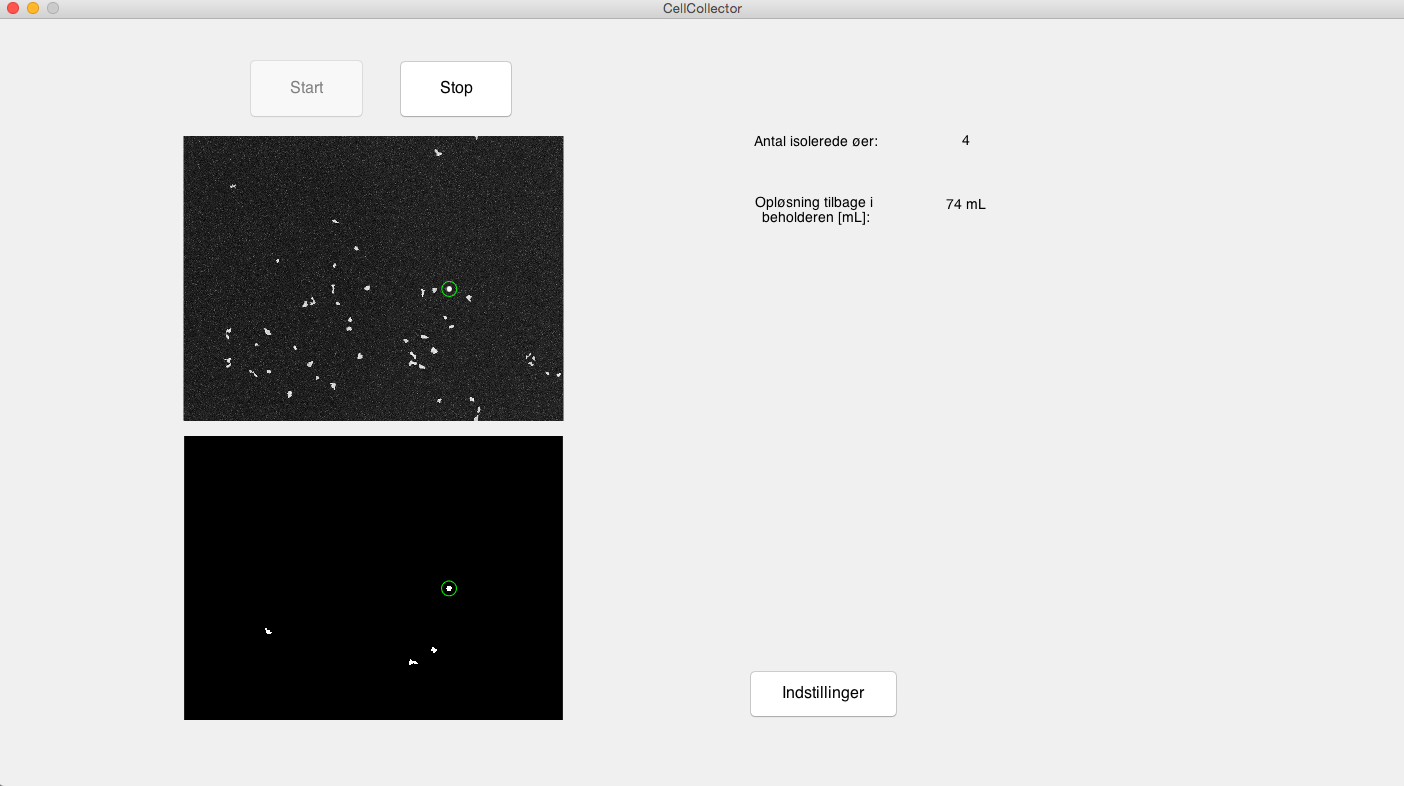
\includegraphics[width=1\textwidth]{billeder/gui_main.png}
	\caption{Brugergrænsefladen på prototypen}
	\label{fig:finalgui}
\end{figure}